\subsubsection{Instrument Signature Removal}
\label{ssec:isr}
The first step in processing \gls{LSSTComCam} images is to correct for the effects introduced by the telescope and detector.
Each sensor and its readout amplifiers can vary slightly in performance, causing images of even a uniformly illuminated focal plane to exhibit discontinuities and shifts due to detector effects.
The \gls{ISR} pipeline aims to recover the original astrophysical signal as best as possible and produce science-ready single-epoch images for source detection and measurement.
A detailed description of the \gls{ISR} procedures can be found in \citet{SITCOMTN-086,2025JATIS..11a1209P}.
\figref{fig:isr_signal_chain} illustrates the model of detector components and readout electronics and their impact on the signal, tracing the process from photons incident on the detector surface to the final quantized values\footnote{The images written to disk by the camera have values that are integers that come from the ADC converting an analog voltage.} recorded in the image files.
The \gls{ISR} \gls{pipeline} essentially ``works backward'' through the signal chain, correcting the integer analog-to-digital units (ADU) raw camera output back to a floating-point number of photoelectrons created in the silicon.
The physical detector, shown on the left in  \figref{fig:isr_signal_chain}, is the source of effects that arise from the silicon itself, such as the dark current and the brighter-fatter effect \citep{doi:10.1088/1538-3873/aab820,2024PASP..136d5003B}.
After the integration time has elapsed, the charge is shifted  to the serial register and read out, which can introduce charge transfer inefficiencies and a clock-injected offset level.
The signals for all amplifiers are transferred via cables to the \gls{REB}, during which crosstalk between the amplifiers may occur.
The \gls{ASPIC} on the \gls{REB} converts the analog signal from the detector into a digital signal, adding both quantization and a bias level to the image.
Although the signal chain is designed to be stable and linear, the presence of numerous sources of non-linearity indicates otherwise.
\begin{figure}[htb]
  \centering
  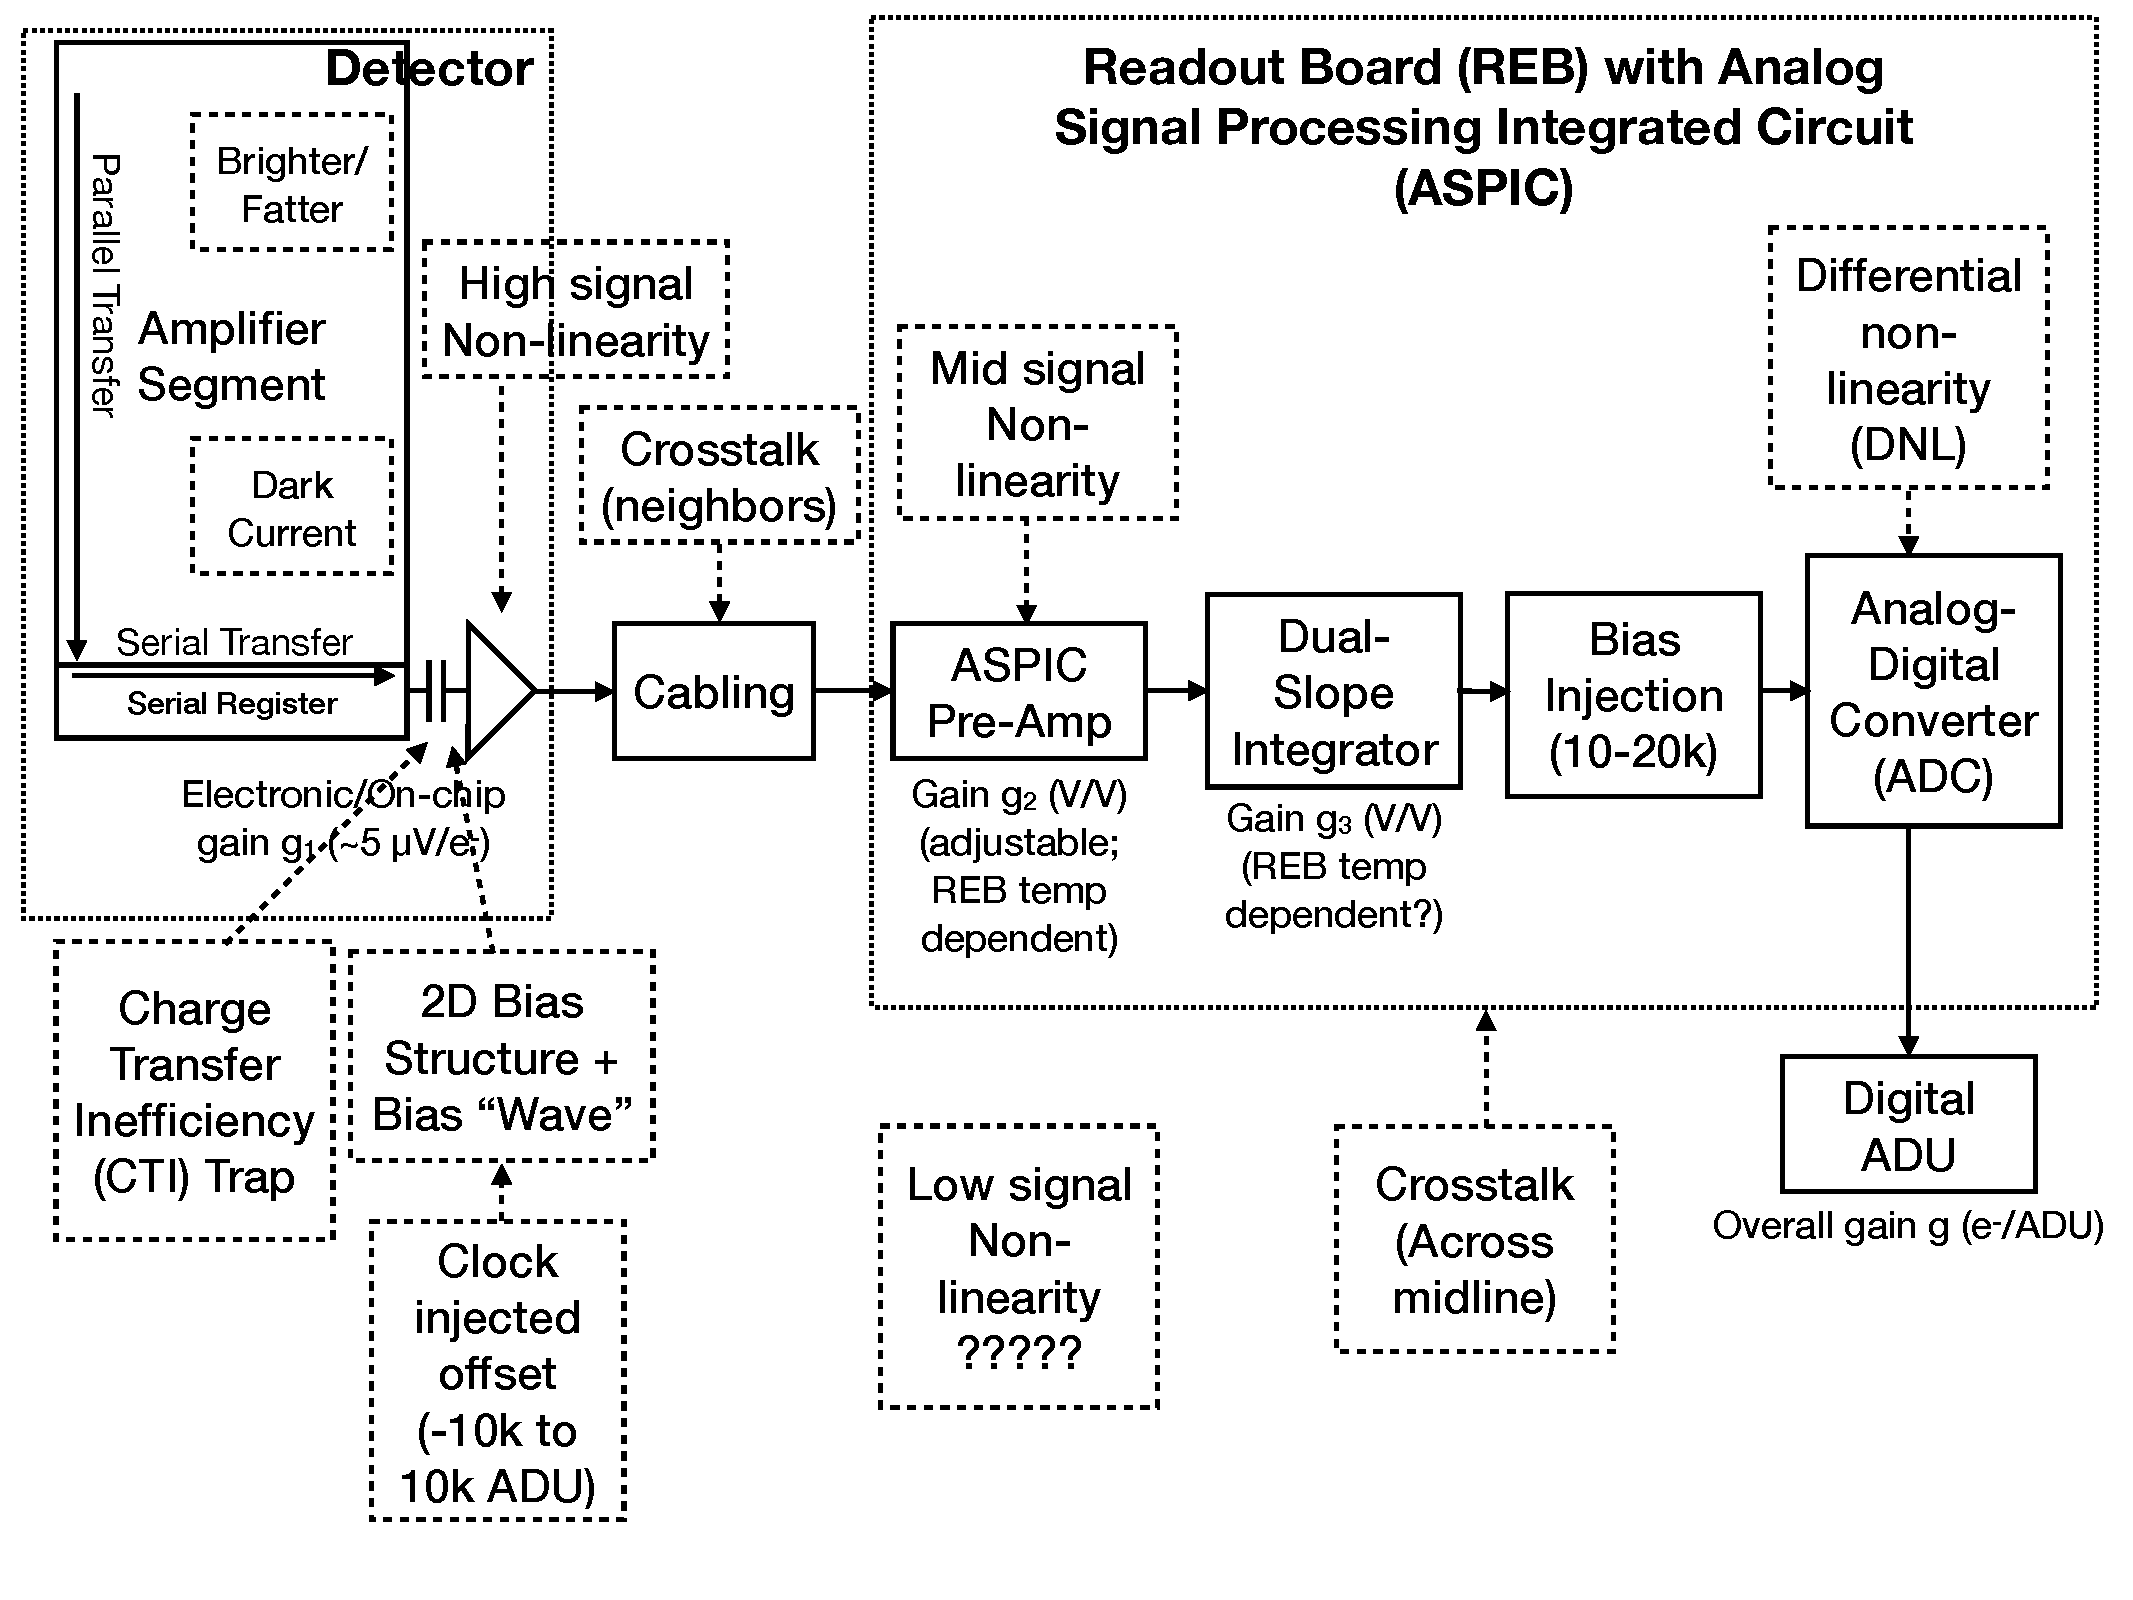
\includegraphics[width=\linewidth]{calibration_boxes_detector_model}
  \caption{The model of the detector and REB components, labeled with the effects that they impart on signal.}
  \label{fig:isr_signal_chain}
\end{figure}

The \gls{ISR} processing pipeline for \gls{DP1} performs, in the following order: \gls{ADU} dithering to reduce quantization effects, serial overscan subtraction, saturation masking, gain normalization, crosstalk correction, parallel overscan subtraction, linearity correction, serial \gls{CTI} correction, image assembly, bias subtraction, dark subtraction, brighter-fatter correction, defect masking and interpolation, variance plane construction, flat fielding, and amplifier offset (amp-offset) correction\footnote{Amp-offset corrections are designed to address systematic discontinuities in background sky levels across amplifier boundaries. The implementation in the LSST Science Pipelines is based on the \texttt{Pan-STARRS} Pattern Continuity algorithm \citep{2020ApJS..251....4W}.}.
Flat fielding for \gls{DP1} was performed using combined flats produced from twilight flats acquired with sufficient rotational dithering to mitigate artifacts from print-through stars, as described in \secref{ssec:flat_field_system}.